\documentclass[border=0pt]{standalone}
\usepackage[T1]{fontenc}
\usepackage{lmodern,amsmath,graphicx,tikz}
\usetikzlibrary{arrows.meta,calc,positioning}
\definecolor{ink}{HTML}{20252C}
\definecolor{blue}{HTML}{0072B2}
\definecolor{raw}{HTML}{C1272D}
\definecolor{green}{HTML}{39775A}
\definecolor{orange}{HTML}{D55E00}
\definecolor{muted}{HTML}{69717A}
\tikzset{every node/.style={font=\fontsize{9}{10.8}\selectfont,text=ink,inner sep=1mm,outer sep=0pt,align=center},
 title/.style={font=\fontsize{9}{10.8}\selectfont\bfseries},
 detail/.style={font=\fontsize{8.5}{10.2}\selectfont,text=muted},
 box/.style={draw=blue!65,fill=blue!3,line width=.65pt,rounded corners=1mm,minimum height=13mm},
 flow/.style={draw=blue,line width=.8pt,shorten <=.5pt,shorten >=.5pt,-{Latex[length=2mm,width=1.3mm]}},
 ref/.style={draw=green,dashed,line width=.7pt}}

\begin{document}
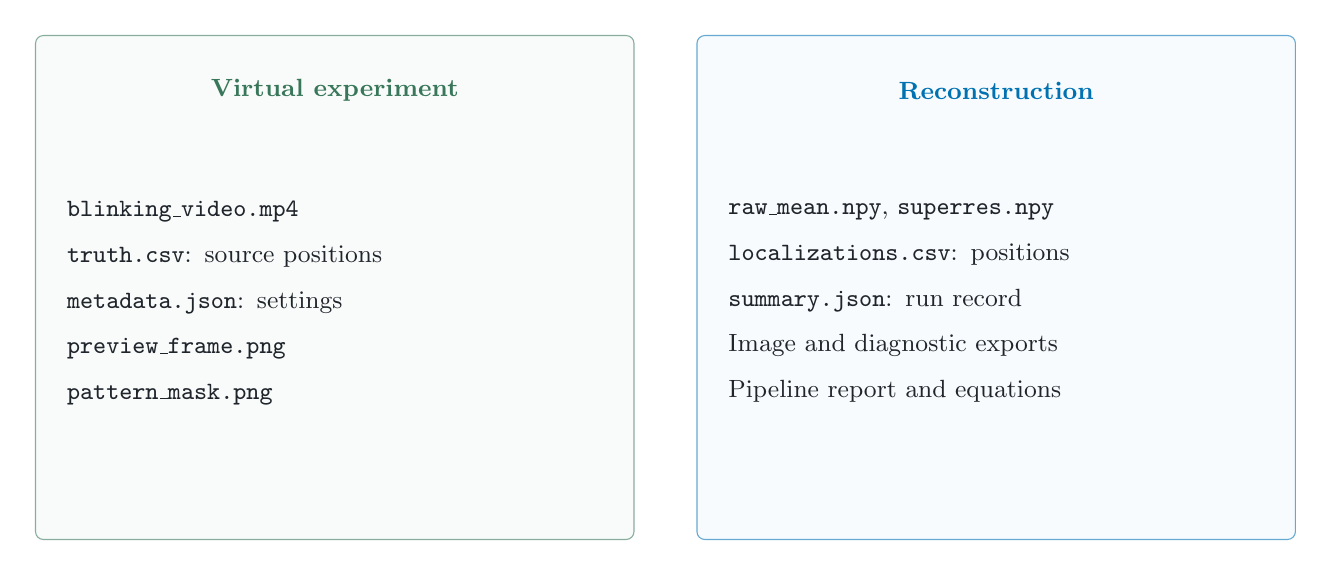
\begin{tikzpicture}[x=1mm,y=1mm]
\path[use as bounding box] (0,0) rectangle (162,66);
\draw[green!60,fill=green!3,rounded corners=1mm] (1,1) rectangle (77,65);
\draw[blue!60,fill=blue!3,rounded corners=1mm] (85,1) rectangle (161,65);
\node[title,text=green] at (39,58) {Virtual experiment};
\node[title,text=blue] at (123,58) {Reconstruction};
\node[align=left,text width=68mm] at (39,31) {\texttt{blinking\_video.mp4}\\[2mm]\texttt{truth.csv}: source positions\\[2mm]\texttt{metadata.json}: settings\\[2mm]\texttt{preview\_frame.png}\\[2mm]\texttt{pattern\_mask.png}};
\node[align=left,text width=68mm] at (123,31) {\texttt{raw\_mean.npy}, \texttt{superres.npy}\\[2mm]\texttt{localizations.csv}: positions\\[2mm]\texttt{summary.json}: run record\\[2mm]Image and diagnostic exports\\[2mm]Pipeline report and equations};
\end{tikzpicture}
\end{document}
